%!TEX root = main.tex

A motivating example is the POS tagging. The goal is to assign a POS tag to each word of a sentence. This tagging is ambiguous, so we will choose a tag according to the context of the word. Words are observed and tags are hidden. We will use a finite state model where tags are states and tagging a sentence reduces to find the most likely state sequence.

\subsection{Markov Chains}

\begin{figure}[htp]
	\centering
	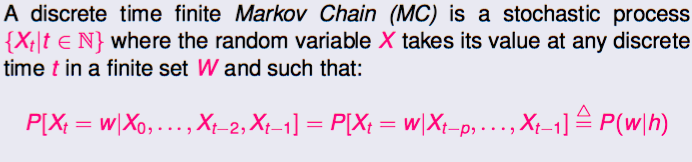
\includegraphics[scale=0.5]{images/22_chains.png}
 	\caption{A Markov chain of order p is a N-Gram model with $N = p+1$. }
\end{figure}

\begin{figure}[htp]
	\centering
	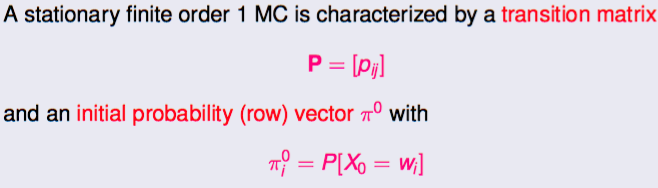
\includegraphics[scale=0.6]{images/23_prob.png}
 	\caption{Transition and initial probabilities.}
\end{figure}


\begin{figure}
\centering
\begin{minipage}{.5\textwidth}
  \centering
  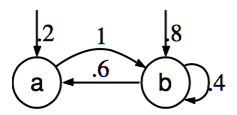
\includegraphics[scale=0.6]{images/24_ex1.png}
\end{minipage}%
\begin{minipage}{.5\textwidth}
  \centering
  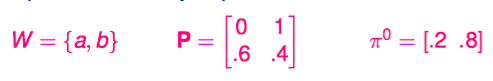
\includegraphics[scale=0.5]{images/25_ex2.png}
\end{minipage}
\end{figure}

The maximal number of states $|W|^p$ grows exponentially with $p$.

\begin{figure}[htp]
	\centering
	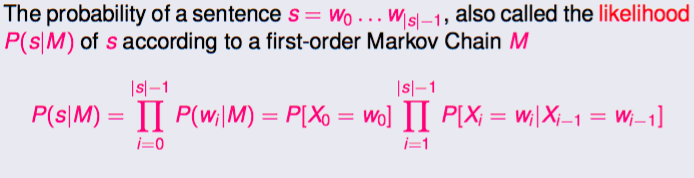
\includegraphics[scale=0.5]{images/26_sentence.png}
 	\caption{A sentence probability for a Markov Chain.}
\end{figure}

\subsection{Hidden Markov Models}

\begin{figure}[H]
	\centering
	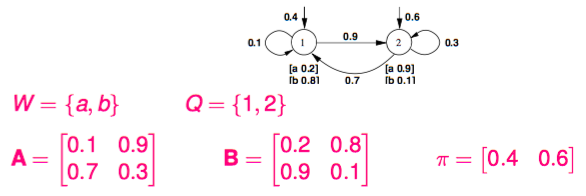
\includegraphics[scale=0.5]{images/27_ex1.png}
\end{figure}

\begin{figure}[H]
	\centering
	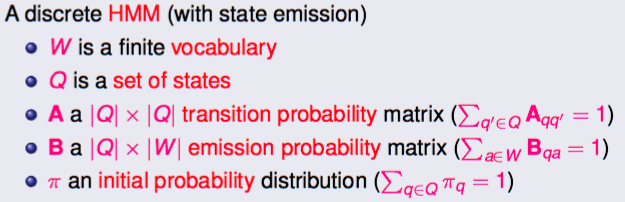
\includegraphics[scale=0.5]{images/28_ex2.png}
\end{figure}

\subsubsection{Path likelihood}
\begin{figure}[htp]
	\centering
	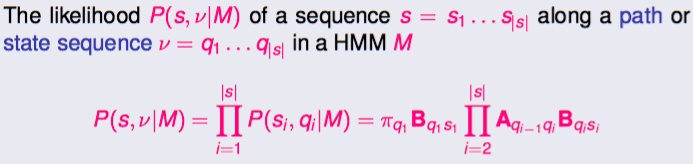
\includegraphics[scale=0.6]{images/29_path.png}
 	\caption{Path likelihood.}
\end{figure}

\subsubsection{Sequence likelihood}
Complicated because $O(|Q|^{|S|})$ possible state sequences ($|Q|$ is number of states and $|S|$ is sequence length).


\subsection{Most likely state sequence}

\begin{figure}[htp]
	\centering
	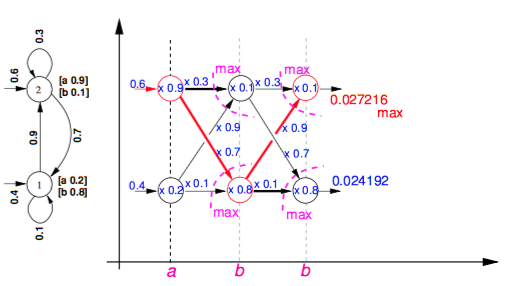
\includegraphics[scale=0.6]{images/30_viterbi.png}
 	\caption{Example.}
\end{figure}

\begin{figure}[htp]
	\centering
	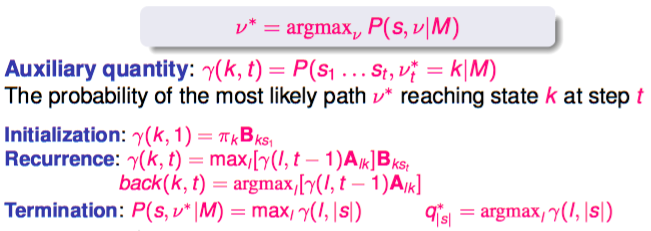
\includegraphics[scale=0.6]{images/31_viterbi.png}
 	\caption{Viterbi decoding (recurrence) Algorithm.}
\end{figure}

\begin{itemize}
	\item $P(s, v^*)$ gives the probability of the optimal path $v^*$;
	\item Computation are done with log (because too small values);
	\item Complexity: $\Theta(m|s|)$;
	\item Path $v^*$ is an alignement between states and words;
	\item $v^*$ can be recovered with the backpointers.
\end{itemize}

\newpage

\subsection{Sequence likelihood}

\begin{figure}[htp]
	\centering
	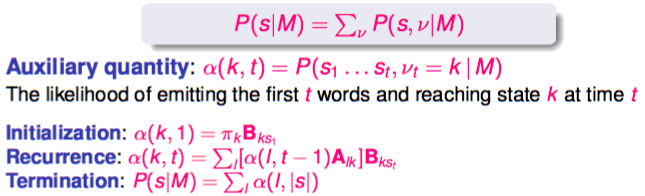
\includegraphics[scale=0.6]{images/32_forward.png}
 	\caption{Forward recurrence, same complexity as viterbi recurrence.}
\end{figure}

\subsection{The learning problem}

Given an HMM structure and several sentences, you must estimate $A$, $B$, $\pi$.

\subsubsection{Supervised}

The learning sentences are annoted with their respective states.

\begin{figure}[htp]
	\centering
	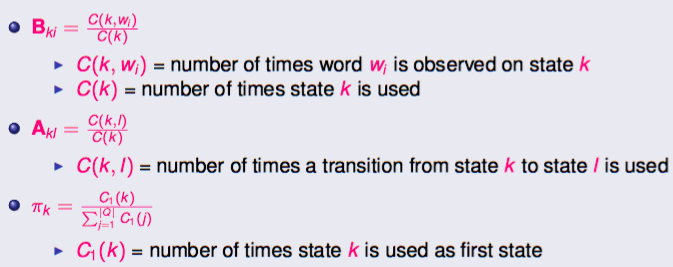
\includegraphics[scale=0.6]{images/33_supervised.png}
 	\caption{Supervised learning.}
\end{figure}


\subsubsection{Unsupervised}

The sentences are not annoted. There is two algorithm. The first one is \textbf{Viterbi training}.

\begin{figure}[htp]
	\centering
	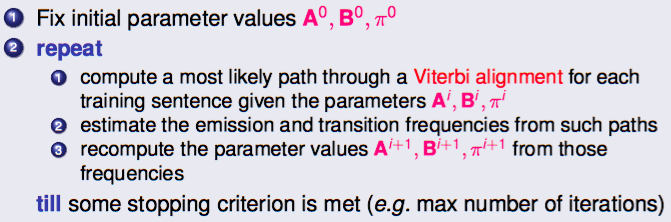
\includegraphics[scale=0.6]{images/34_viterbi.png}
 	\caption{Viterbi learning.}
\end{figure}

The second is \textbf{Forward-Backward} or \textbf{Braaum-Welch} algorithm. Viterbi training is an approximation as it considers that each training sentence is generated along a single path. A more accurate estimation is obtained if one considers all possible paths to generate each sentence.

\begin{itemize}
	\item actual frequencies ($C(k, w_i)$, $C(k)$, $C(k, l)$, \dots ), are replaced by expected frequencies;
	\item   special case of expectation-maximization (EM) procedure
\end{itemize}

Viterbi and Baum-Welch training are both sensitive to parameter initialization.



